\chapter{Doświadczenie}
Przeprowadzone doświadczenie polega na porównaniu dostępnych w środowisku Microsoft Azure algorytmów klasyfikacji danych dwu-klasowych wraz z algorytmem stworzonym na potrzeby pracy inżynierskiej o tytule ''\textit{Wykorzystanie algorytmów genetycznych w systemach wykrywania intruzów w sieciach komputerowych}''\cite{Blyszcz2022} oraz z algorytmem DANet\cite{Chen2022}. Doświadczenie przebiegało według \refsource{schematu}{fig:sch-prac}.

\begin{figure}[H]
    \centering
    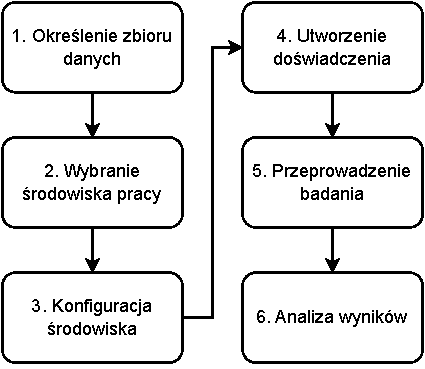
\includegraphics[width=0.9\textwidth]{images/schemat_pracy}
    \captionsource{Schemat przebiegu doświadczenia}{Opracowanie własne}
    \label{fig:sch-prac}
\end{figure}

\section{Metodologia badwcza}
Przyjęta w projekcie metodologia badawcza została określona w poniższej \refsource{tabeli}{tab:met-bad}. Przyjęta metodologia ma za zadanie określić jakoś porównywanego algorytmu.

\begin{table}[H]
    \centering
    \captionsource{Metodologia badawcza}{Opracowanie własne}
    \begin{tabular}{|L{\textwidth}|}
        \hline
        \textbf{Problem badawczy:} \\
        Czy algorytm klasyfikacji danych utworzony w ramach pracy inżynierskiej może konkurować z rozwiązaniami dostępnymi w środowiskach komercyjnych \\ \hline

        \textbf{Pytania badawcze:} \\
        \begin{enumerate}
            \item Czy algorytm jest konkurencyjny pod względem wybranych metry:
            \begin{itemize}
                \item dokładność algorytmu
                \item czas działania
                \item precyzja
                \item czułość
                \item f1
                \item auc
            \end{itemize}
        \end{enumerate} \\ \hline

        \textbf{Hipotezy:} \\
        \begin{enumerate}
            \item Nie ma istotnej różnicy w uzyskanej ''\textit{dokładności}'' między algorytmami.
            \item Nie ma istotnej różnicy w uzyskanej ''\textit{czułości}'' między algorytmami.
            \item Nie ma istotnej różnicy w uzyskanej ''\textit{precyzji}'' między algorytmami.
            \item Nie ma istotnej różnicy w uzyskanym ''\textit{auc}'' między algorytmami.
            \item Nie ma istotnej różnicy w uzyskanej ''\textit{f1}'' między algorytmami.
            \item Nie ma istotnej różnicy w uzyskanym ''\textit{czasie działania}'' między algorytmami.
        \end{enumerate} \\ \hline
    \end{tabular}
    \label{tab:met-bad}
\end{table}

\section{Dane}
Zbiór danych został przygotowany przez Kanadyjski Instytut Cyberbezpieczeństwa działający przy Uniwersytecie Nowy Brunszwik za pomocą narzędzia CICFlowMeter\cite{Ahlashkari2022}. Zbiór zawiera 79 cech ruchu sieciowego do których zaliczyć można: etykietę, czas trwania przesyłu, minimalną długość pakietu zwrotnego, maksymalną długość pakietu zwrotnego, port docelowy, długość pakietów. Zbiór pozwala na określenie czy ruch sieciowy jest życzliwy \trans{ang. BENING}, czy nieżyczliwy (różne możliwe formy ataku na sieć). Dodatkowo zbiór został podzielony na pięć dni roboczych: poniedziałek 3.07.2017 - piątek 7.07.2017. Dane z poniedziałku zawierają jedynie ruch życzliwy, zaś w pozostałe dni zostały zasymulowane ataki na sieć komputerową\cite{Blyszcz2022, unbkaggle}.

\section{Środowisko programistyczne}
Jako środowisko programistyczne zostało wybrane Azure Machine Learning Studio z powodu możliwości uniezależnienia obliczeń od komputera lokalnego, dodatkowo platforma umożliwia łatwy sposób na tworzenie skomplikowanych potoków zadań, które składają się z komponentów wielokrotnego użytku. Każdy komponent uruchamia się w środowisku odizolowanym od pozostałych operacji. Dzieje się tak dzięki wykorzystaniu wielo węzłowych klastrów obliczeniowych, bazujących na oprogramowaniu Docker, klastry te mogą skalować się w zależności od potrzeb oraz dostępnej jednostki\cite{MicrosoftLearn2023}.
\\ \\
Całe doświadczenie zostało odwzorowane w graficznym potoku narzędzia ''\textit{Projektant}'' oraz przedstawione na \refsource{zdjęciu}{fig:pipeline}.

\begin{landscape}
\begin{figure}[H]
    \centering
    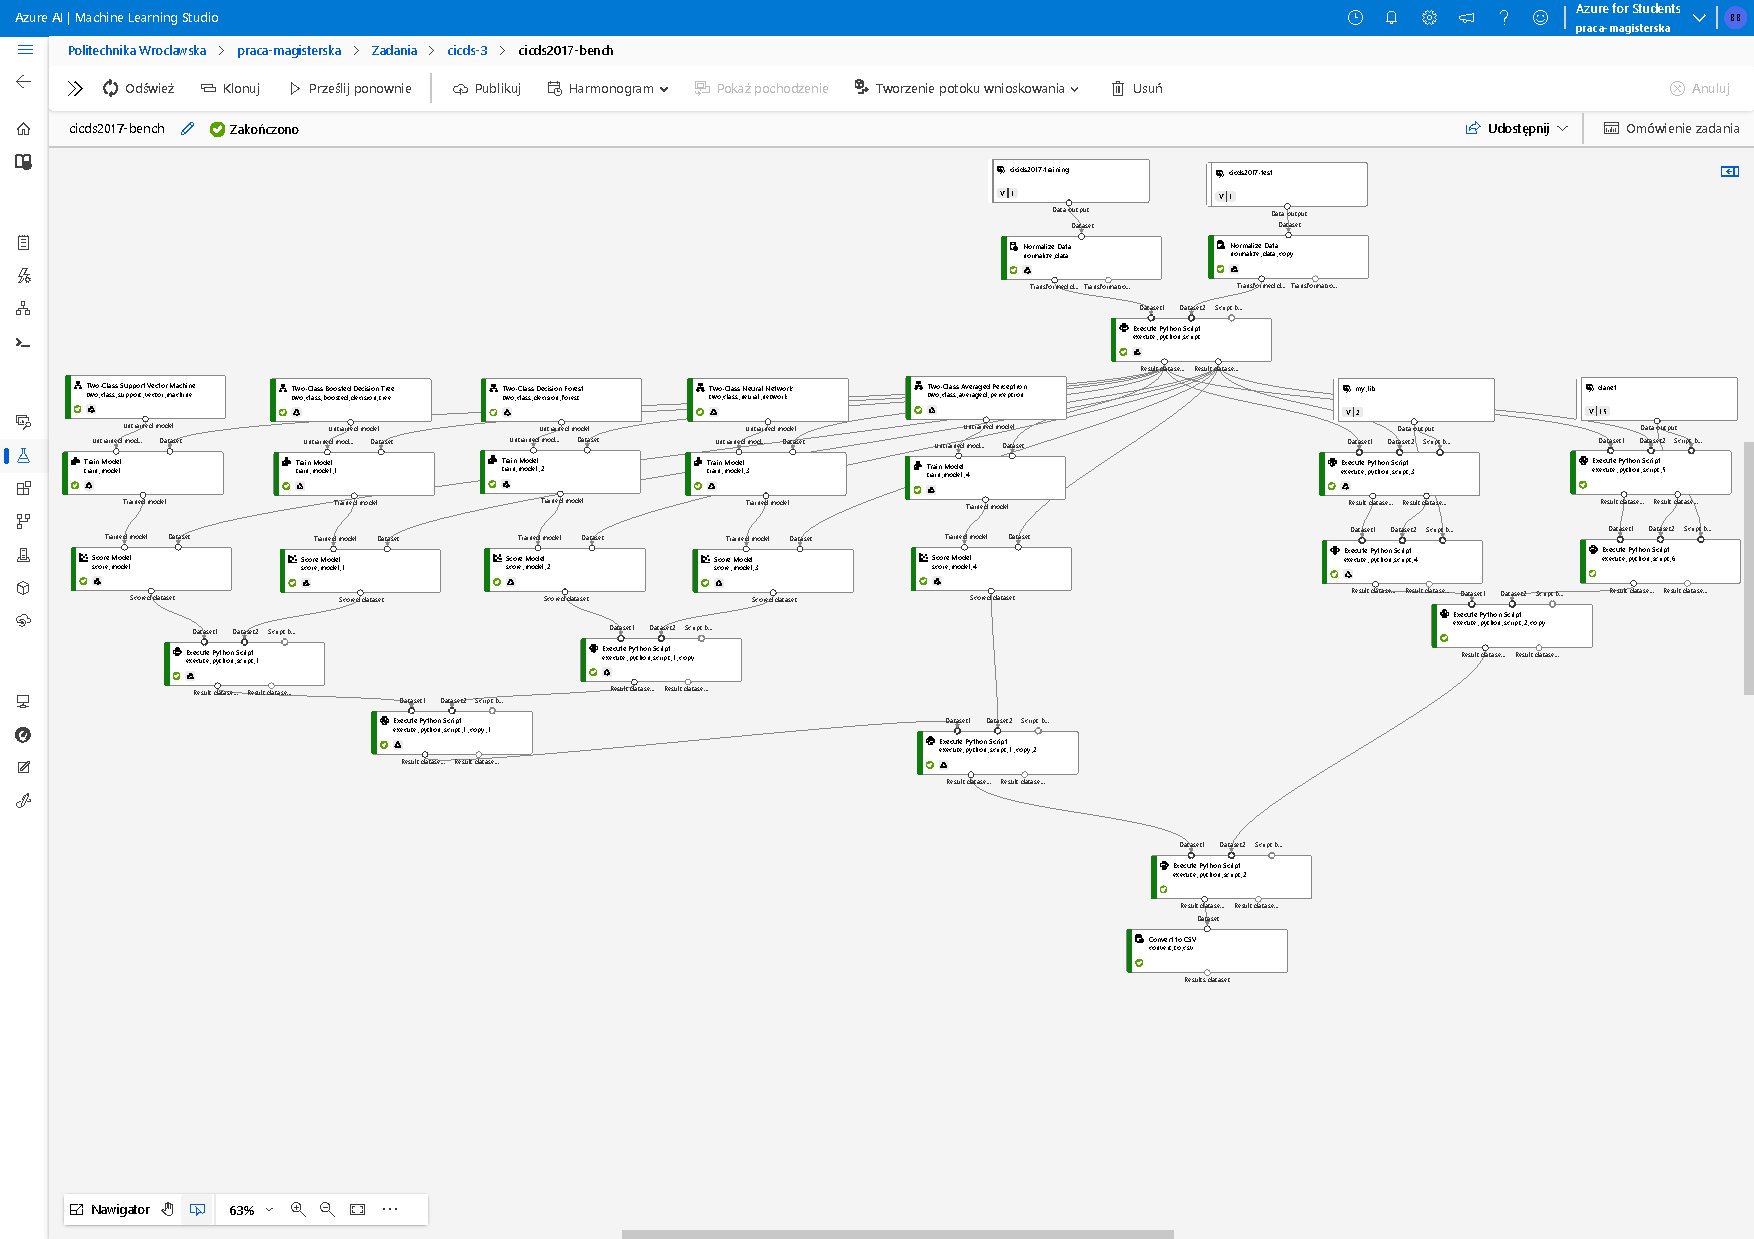
\includegraphics[height=0.9\textwidth]{images/pipeline}
    \captionsource{Potok zadań}{Opracowanie własne}
    \label{fig:pipeline}
\end{figure}
\end{landscape}

\section{Algorytmy}
W trakcie eksperymenty zastosowano różne algorytmy klasyfikacji danych. Charakterystyczną cechą tych algorytmów jest klasyfikacja ukierunkowana na 2 kategorie wejściowe. W tym wypadku są to kategorie ruchu sieciowego: [\textbf{BENIGN} \trans{pl. życzliwy}, \textbf{Other} \trans{pl. inne}], gdzie inne to pozostałe typy ruchu sieciowego.

\subsection{Two-Class Support Vector Machine}
Algorytm SVM ma za zadanie znaleźć hiperpłaszczyznę w przestrzeni K-wymiarowej (K - liczba cech), która rozdziela zbiory punktów odpowiadających różnym klasom. W pierwszej kolejności szuka się separatora między klasami, a następnie przekształca się dane w taki sposób, by można przekształcić separator w hiperpłaszczyznę\cite{IBM}. Sposób działania został zobrazowany za pomocą \refsource{wykresów}{fig:svm-schem}. Część \refsource{potoku}{fig:pipeline} odpowiedzialnego za SVM to \refsource{schemat}{fig:svm-pipe}.

\begin{figure}[H]
    \begin{subfigure}[m]{0.45\textwidth}
        \centering
        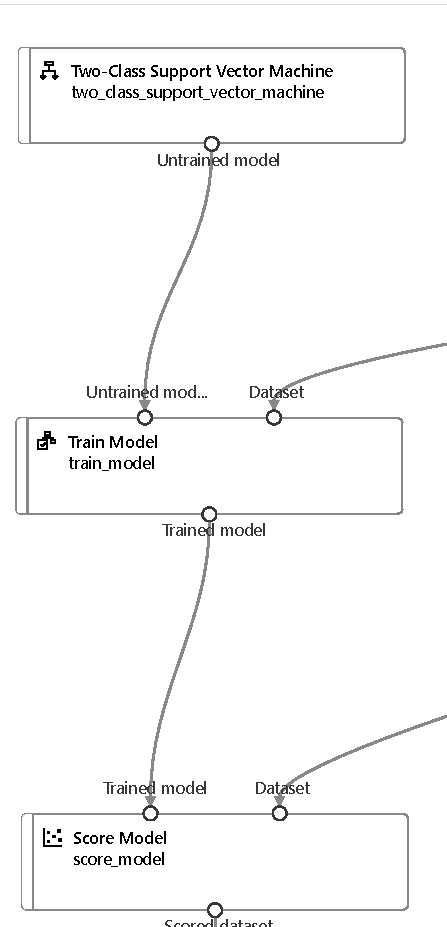
\includegraphics[width=\textwidth]{images/svm_pipe}
        \captionsource{Potok zadań dla modelu \textit{Two-Class Support Vector Machine}}{Opracowanie własne}
        \label{fig:svm-pipe}
    \end{subfigure}
    \hfill
    \begin{subfigure}[m]{0.45\textwidth}
        \centering
        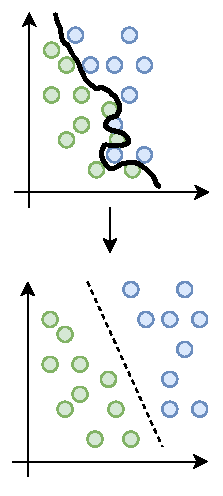
\includegraphics[width=\textwidth]{images/svm}
        \captionsource{Schemat SVM}{\cite{Statsoft}}
        \label{fig:svm-schem}
    \end{subfigure}
\end{figure}

\subsection{Two-Class Boosted Decision Tree}
Jest to algorytm drzewa decyzyjnego oparty o algorytm LightGBM. Dzięki zastosowaniu tego podejścia algorytm oparty o drzewo decyzyjne działa szybciej oraz ma mniejszą złożoność obliczeniową. Algorytm ten działa na zasadzie doboru odpowiedniego liścia zamiast jak w przypadku klasyzcnych algorytmów opartych na drzewie, wyboru odpowiedniej warstwy warstwy\cite{LightGBM}. Sposób podejścia liściastego został ukazany na \refsource{schemacie}{fig:leaf}. Model wykorzystywany w Azure ML został ukazany na \refsource{rysunku}{fig:dt-pipe}.
\begin{figure}[H]
    \begin{subfigure}[m]{0.3\textwidth}
        \centering
        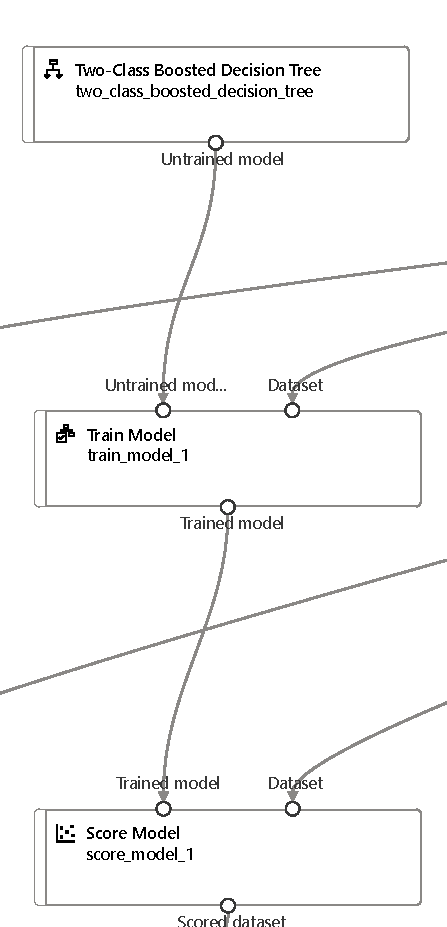
\includegraphics[width=\textwidth]{images/dt_pipe}
        \captionsource{Potok zadań dla modelu \textit{Two-Class Boosted Decision Tree}}{Opracowanie własne}
        \label{fig:dt-pipe}
    \end{subfigure}
    \hfill
    \begin{subfigure}[m]{0.66\textwidth}
        \begin{subfigure}[m]{\textwidth}
            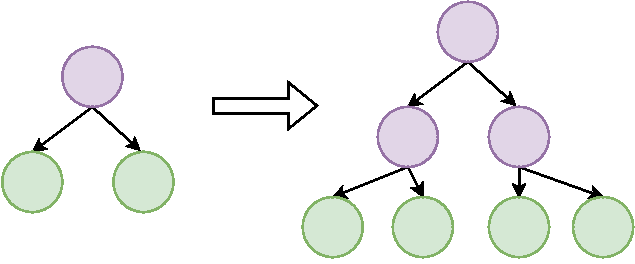
\includegraphics[width=\textwidth]{images/level-wise}
        \end{subfigure}
        \begin{subfigure}[m]{\textwidth}
            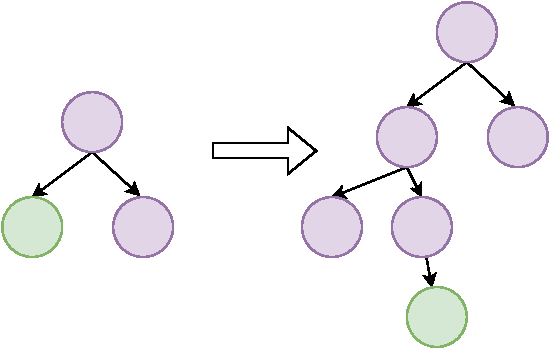
\includegraphics[width=\textwidth]{images/leaf-wise}
        \end{subfigure}
        \captionsource{Sposób działania algorytmu}{\cite{LightGBM}}
        \label{fig:leaf}
    \end{subfigure}
\end{figure}

\subsection{Two-Class Decision Forest}
Las decyzyjny to algorytm którego wynik opiera się o agregację wyników wielu drzew decyzyjnych. Uzyskanie wyniku zależy od algorytmu trenowania lasu. Przykładowo w klasyfikacji losowym lasem wieloklasowym \trans{ang. Multi-class random forest classification}, każde drzewo głosuje na jedną klasę i ta, która zostanie wybrana większością głosów zostaje uznana za wynikową\cite{Google}. Model wykorzystany w Azure ML jest pokazany na \refsource{modelu}{fig:df-pipe}

\begin{figure}[H]
    \centering
    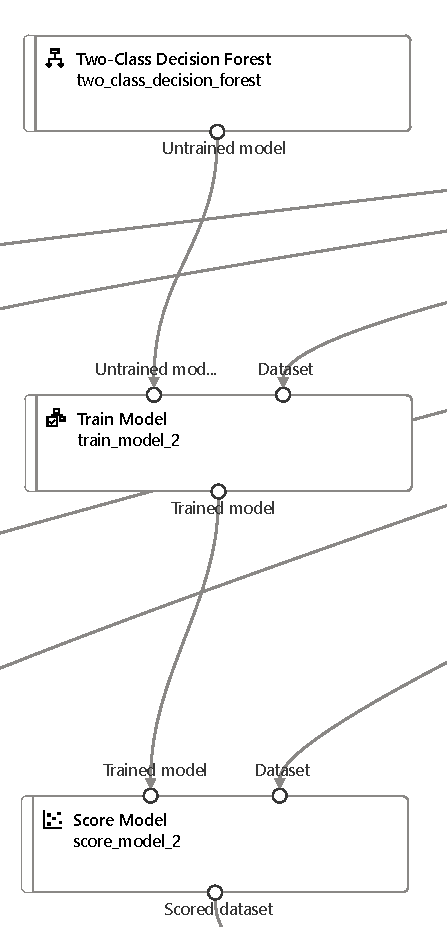
\includegraphics[width=0.3\textwidth]{images/df_pipe}
    \captionsource{Potok zadań dla modelu \textit{Two-Class Decision Forest}}{Opracowanie własne}
    \label{fig:df-pipe}
\end{figure}



\subsection{Two-class Neural Network}
Jest to sieć neuronowa składająca się w tym wypadku z warstwy wejściowej, trzech warstw ukrytych każda po 100 węzłów, oraz z warstwy wyjściowej. Przykładowa sieć neuronowa została zobrazowana na \refsource{schemacie}{fig:neural-network}. Moduł wykrozystany w Azure ML ukazano na \refsource{rysunku}{fig:nn-pipe}.

\begin{figure}[H]
    \centering
    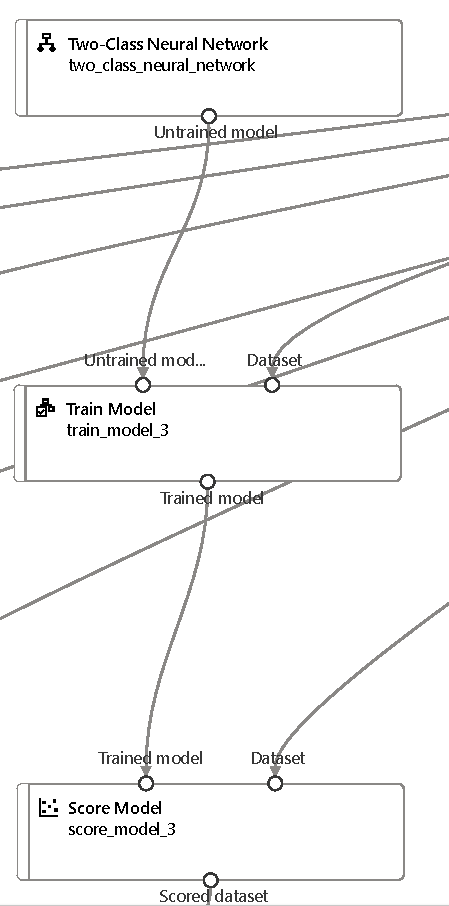
\includegraphics[width=0.3\textwidth]{images/nn_pipe}
    \captionsource{Potok zadań dla modelu \textit{Two-Class Neural Network}}{Opracowanie własne}
    \label{fig:nn-pipe}
\end{figure}

\subsection{Two-Class Average Perceptron}
Jest to najprostsza odmiana sieci neuronowej czyli pojedynczy perceptron, który jest matematycznym modelem neuronu. Składa się on z \textit{n} wejść, takiej samej ilości wag, progu $\Theta$, sumatora, funkcji aktywującej i wyjścia. Został zobrazowany na \refsource{schemacie}{fig:neuron}. Może służyć za prosty klasyfikator binarny, albo za regresor. Model wykorzystany w Azure ML ukazano na \refsource{zdjęciu}{fig:ap-pipe}.
\begin{figure}[H]
    \centering
    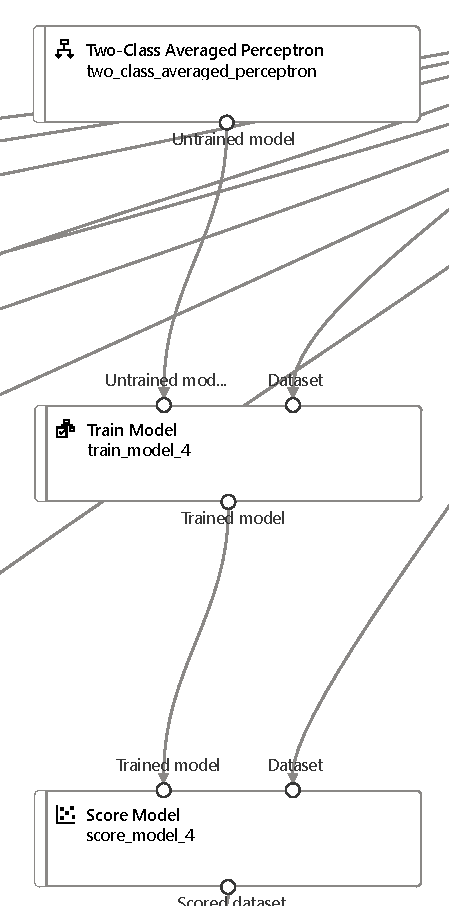
\includegraphics[width=0.3\textwidth]{images/ap_pipe}
    \captionsource{Potok zadań dla modelu \textit{Two-Class Average Perceptron}}{Opracowanie własne}
    \label{fig:ap-pipe}
\end{figure}

\subsection{Autorskie rozwiązanie}
Algorytm ten polega na połączeniu algorytmu genetycznego (GA) wraz z klasyfikatorem naiwnym Bayesa wykorzystującego rozkład Gaussa (GNB). Zadaniem algorytmu genetycznego jest znalezienie naistotniejszych cech w zbiorze tabelarycznym, które pozwolą na zmniejszenie wymiarowości danych, oraz na zmniejszenie kosztów obsługi samego klasyfikatora w późniejszych etapach testowania, ze względu na zmniejszoną ilość danych wymaganych do przetworzenia. GA wykrozystywał w metodzie \textbf{fitness} algorytm GNB w celu określenia dopasowania danych. Zadaniem GNB było znalezienie najlepszej dostępnej kombinacji cech, któe pozwalały na uzyskanie najlepszego dopasowania \cite{Blyszcz2022}. Model wykorzystywany w Azure ML różni się od gootwych modeli tym, że dołączono do niego bibliotekę napisaną w języku python, która zawiera kod wykorzystywany w pracy inżynierskiej autora\cite{Suvres2023}.
\begin{figure}[H]
    \centering
    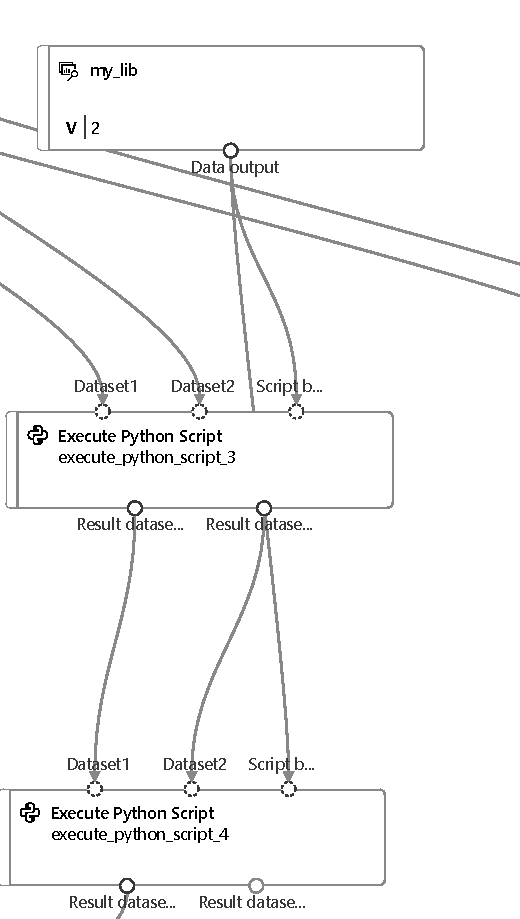
\includegraphics[width=0.3\textwidth]{images/ga_pipe}
    \captionsource{Potok zadań dla modelu}{Opracowanie własne}
    \label{fig:ga-pipe}
\end{figure}

\subsection{DANet}
Twórcy tego algorytmu wprowadzają dodatkową warstwę abstrakcyjną o nazwie ''\textit{Abstract Layer}''. Wartswy te budują sieć o nazwie ''\textit{Deep Abstract Network}'' (DANet). Zadanie dodatkowych warstw jest grupowanie cech w skorelowanych zbiorach. Zbiory te budują sieć powiązań między sobą w formie sieci semantycznej. Gdy sieć semantyczna jest zbudowana w ostatnim kroku wykonywana jest klasyfikacja w trzywarstwowej sieci perceptronów \trans{ang. Multilayer Perceptron network} (MLP)\cite{Chen2022, Danet}. Model znajdujący się z Azure ML został przedstawiony na \refsource{zdjęciu}{fig:danet-pipe}, zaś sposób działania ukazano na \refsource{schematach}{fig:danet-abst}.

\begin{figure}[H]
    \begin{subfigure}[m]{0.49\textwidth}
        \centering
        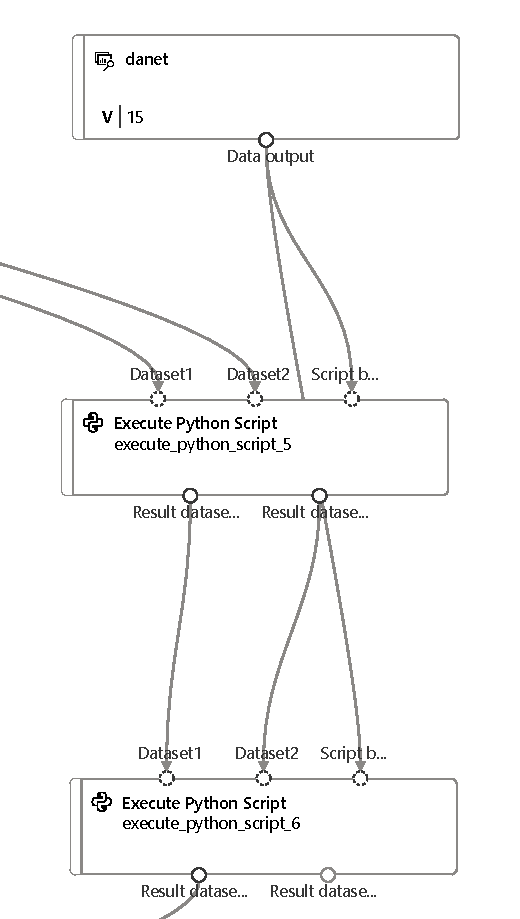
\includegraphics[width=0.4\textwidth]{images/danet}
        \captionsource{Potok zadań dla modelu \textit{DANet}}{Opracowanie własne}
        \label{fig:danet-pipe}
    \end{subfigure}
    \hfill
    \begin{subfigure}[m]{0.49\textwidth}
        \begin{subfigure}[m]{\textwidth}
            \centering
            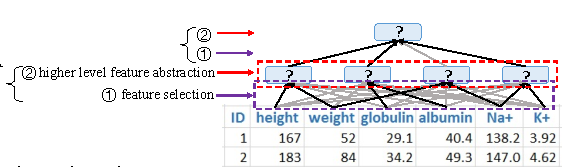
\includegraphics[width=\textwidth]{images/danet_1}
        \end{subfigure}
        \begin{subfigure}[m]{\textwidth}
            \centering
            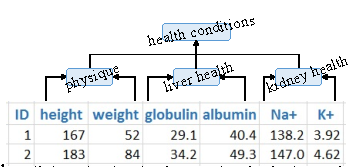
\includegraphics[width=\textwidth]{images/danet_2}
        \end{subfigure}
        \captionsource{Sposób działania DANet}{\cite{Chen2022}}
        \label{fig:danet-abst}
    \end{subfigure}

\end{figure}




